\section{选择结构}
在此之前我们遇到的代码都是顺序结构的,程序一个接一个地执行一系列操作。仅用顺序结构是不能完成复杂工作的,比如根据一定的条件,作出不同的反应。这时我们就需要用到选择结构了。\par
\lstinline@if@-\lstinline@else@ 结构是最常用的选择结构,而 \lstinline@switch@-\lstinline@case@ 结构在处理特定的条件判断时,会更加高效。本节我们就来介绍这两种结构。\par
\subsection*{\lstinline@if@-\lstinline@else@ 结构}
\lstinline@if@-\lstinline@else@ 结构的基本格式是这样的:
\begin{lstlisting}
    if (<条件>) { //if是必需的
        <若干操作>;
    }
    else { //如果不需要else部分,可以不写
        <若干操作>;
    }
\end{lstlisting}
其中的 \lstinline@<条件>@ 要么是一个 \lstinline@bool@ 数据,要么是可以隐式类型转换为 \lstinline@bool@ 数据的表达式。\par
这个结构其实不复杂,我说一遍你就懂了:如果 \lstinline@<条件>@ 为 \lstinline@true@,那么程序就会执行 \lstinline@if@ 块内的代码,跳过 \lstinline@else@ 块内的代码;如果 \lstinline@<条件>@ 为 \lstinline@false@,那么程序就会跳过 \lstinline@if@ 块内的代码,执行 \lstinline@else@ 块内的代码。当然,如果只有 \lstinline@if@ 块而无 \lstinline@else@ 块,规则就更简单了。\par
初学者一般都会见过这样的问题:输入一个正整数,要求程序判断它是奇数还是偶数,并输出相应的内容。我们就用 \lstinline@if@-\lstinline@else@ 结构来设计这样一个程序。在设计之初,我们需要想清楚一个问题:如何判断一个正整数的奇偶?\par
我们希望有一个表达式,它要么是 \lstinline@bool@ 类型的,要么可以通过布尔转换成为 \lstinline@bool@ 类型,并且能提供``某正整数是奇数还是偶数''这个信息。这里我们选择取模运算,因为一个正整数在对 \lstinline@2@ 取模运算后得到的值只能是 \lstinline@0@ 或 \lstinline@1@——如果这个数是奇数,那么得到 \lstinline@1@;如果是偶数,那么得到 \lstinline@0@。\par
那么有了模运算的结果之后,如何把它表达成一个``条件''呢?这里我们可以使用两种方法:其一是直接把它作为条件,这个运算的结果会隐式转换为 \lstinline@bool@ 类型,奇数意味着 \lstinline@true@,偶数意味着 \lstinline@false@;第二种方法是用相等性运算符 \lstinline@==@\footnote{前面介绍过,当相等性运算符的左右操作数相等时,返回值为 \lstinline@true@;不相等时,返回值为 \lstinline@false@。},我可以用计算结果和 \lstinline@1@ 比较,等于 \lstinline@1@ 意味着 \lstinline@true@;不等于 \lstinline@1@ 就意味着 \lstinline@false@。\par
好,到这里我们已经想清楚了关键部分,那么接下来我们梳理一下我们的程序需要做什么:
\begin{enumerate}
    \item 定义整型变量(可以使用 \lstinline@int@,或者考虑到输入一定是正数而使用 \lstinline@unsigned@),以便后续输入。
    \item 输入这个数。
    \item 再定义一个数,用来保存这个数对 \lstinline@2@ 取模的值。
    \item 写一个选择结构(\lstinline@if@-\lstinline@else@),根据上一步的值是否等于 \lstinline@1@ 来采取不同的操作。(这里采用第二种方法)
\end{enumerate}
有了基本的设计思路之后,我们可以开始写代码了。\par
首先,定义整型变量。我们可以任意起名,但最好起一些有实际含义的名字,这样我们一眼就能知道它是什么,代表什么。比如说,我们就给它起名叫 \lstinline@num@ 吧。
\begin{lstlisting}
    int num; //也可以用unsigned
\end{lstlisting}
接下来是输入部分,很简单,用 \lstinline@cin>>@ 就可以了。
\begin{lstlisting}
    cin >> num; //输入num的值
\end{lstlisting}
然后我们定义一个新的变量,可以叫 \lstinline@mod@,来保存模值。因为这个模值不需要改变,我们可以选择将其定义为 \lstinline@const@ 常量,来防止误改动。
\begin{lstlisting}
    const int mod {num % 2}; //num模除2的值;也可以不用const
\end{lstlisting}\par
最后是整个程序最关键的部分:选择结构。我们以 \lstinline@mod==1@ 作为条件,在这个 \lstinline@if@ 块内让程序输出 \lstinline@"奇数"@,而在 \lstinline@else@ 块内让程序输出 \lstinline@"偶数"@。
\begin{lstlisting}
    if (mod == 1) { //如果mod为1满足,mod==1返回值就是true,执行此段
        cout << "奇数"; //输出"奇数"
    }
    else {
        cout << "偶数"; //输出"偶数"
    }
    \end{lstlisting}
    这个程序的流程图如图3.7所示。可以看出,前面部分是顺序结构,后面部分是选择结构。\par
    \begin{figure}[htbp]
        \centering
        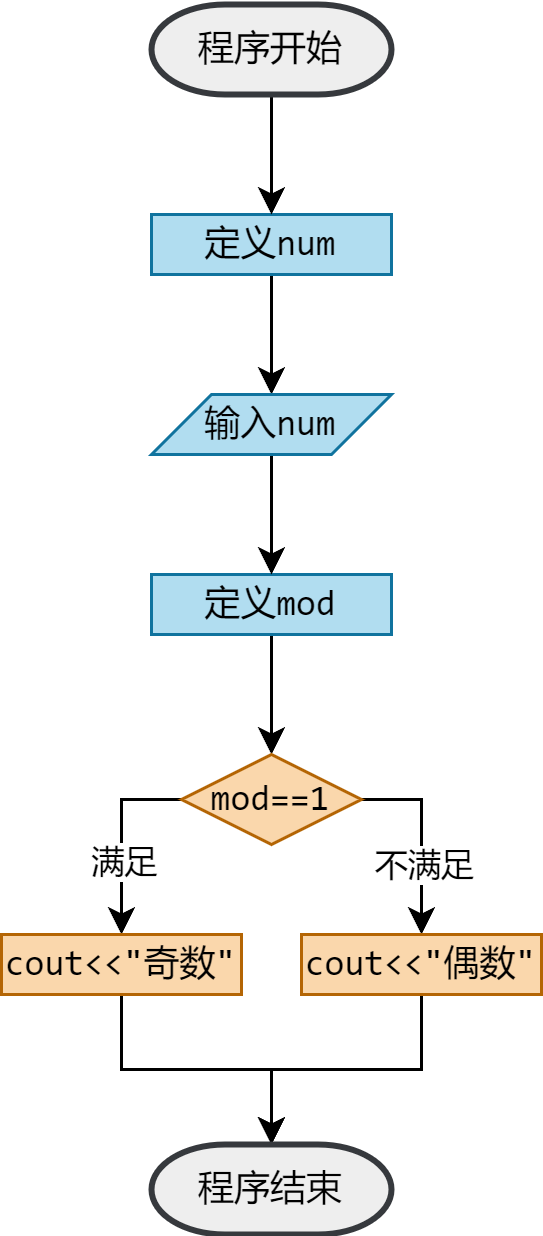
\includegraphics[width=0.3\textwidth]{../images/generalized_parts/03_structure_of_odd_or_even_300.png}
        \caption{奇偶判断程序流程图}
    \end{figure}
最后Ctrl+V一下文件包含等等乱七八糟的代码,就是这样:
\lstinputlisting[caption=\texttt{odd\_or\_even.cpp},label=lst:oddoreven]{../code_in_book/3.2/odd_or_even.cpp}
读者可以自行测试一下,例如输入\texttt{1},程序就会给出输出 \texttt{奇数};输入\texttt{2},程序就会给出输出 \texttt{偶数}。\par
如果甲方有什么其它的奇怪要求,比如``如果是偶数就输出,如果是奇数就不输出'',这时我们就只需要为偶数部分写一个 \lstinline@if@ 块即可,没有必要再写 \lstinline@else@ 块,代码可以这样写:
\begin{lstlisting}
    if (mod == 0) { //注意,判断条件是mod是否为0
        cout << "偶数"; //mod为0说明它是偶数
    } //奇数时什么也不做,那就不需要写else了
\end{lstlisting}
\subsubsection{多路分支的选择结构}
刚才接触到的选择结构是两路分支的,我们可以用一个简单的 \lstinline@if@-\lstinline@else@ 结构来实现这样的功能。但是有些时候我们需要实现更复杂的多路分支。现在我们需要写一个程序,输入单个字符,并判断它是``大写字母''``小写字母''``数字''还是``其它'',那么我们要怎么做呢?\par
首先,我们要知道我们应该用什么样的``判断条件''。如何判断一个字符(起个名字,\lstinline@ch@)是大写字母呢?或许我们可以连用逻辑或来构成一个表达式
\begin{lstlisting}
    if (ch == 'A' || ch == 'B' || ch == 'C' || <此处省略23个>)
\end{lstlisting}
但这样写毕竟还是太麻烦了。我们可以用下面的简单方法来实现:
\begin{lstlisting}
    if (ch >= 'A' && ch <= 'Z')
\end{lstlisting}
还记得我们之前反复提及的ASCII码值吗?\lstinline@'A'@ 到 \lstinline@'Z'@ 在ASCII码表里是连续排列的,如果 \lstinline@ch@ 是26个大写字母之一,那么它一定在大于等于 \lstinline@'A'@ 且小于等于 \lstinline@'Z'@ 的范围内;相反,如果它不是26个大写字母之一,那么它一定不在这个范围内。同样的道理,我们可以用 \lstinline@ch>='a'&&ch<='z'@ 来判断它是不是小写字母,用 \lstinline@ch>='0'&&ch<='9'@ 来判断它是不是数字。\par
关于条件,我们想清楚了,那么如何实现多路分支呢?我们可以看一下这段代码的实现方式:
\begin{lstlisting}
    if (ch >= 'A' && ch <= 'Z') { //判断是否为大写字母
        cout << "大写字母";
    }
    else if (ch >= 'a' && ch <= 'z') { //判断是否为小写字母
        cout << "小写字母";
    }
    else if (ch >= '0' && ch <= '9') { //判断是否为数字
        cout << "数字";
    }
    else { //其它情况
        cout << "其它";
    }
\end{lstlisting}\par
有些参考资料将其称为 \lstinline@if@ - \lstinline@else if@ - \lstinline@else@ 结构,以 \lstinline@if@ 加条件为开头,中间全用 \lstinline@else if@ 加条件的形式,结尾用 \lstinline@else@。\par
但是以我个人的观点来看,实际上并没有 \lstinline@else if@ 这个关键字。它是 \lstinline@else@ 嵌套了 \lstinline@if@ 的结构,本质上只是对 \lstinline@if@-\lstinline@else@ 结构的一种特殊应用。这段代码与下面的代码并无任何区别\footnote{与Python等一些语言不同,C++对代码的缩进、换行和标识符间的空格几乎没有任何限制,所以缩进的修改、换行的使用,乃至特定情况下是否套花括号 \lstinline@\{\}@ 都不会对编译造成影响。}:
\begin{lstlisting}
    if (ch >= 'A' && ch <= 'Z') {
        cout << "大写字母";
    }
    else
        if (ch >= 'a' && ch <= 'z') {
            cout << "小写字母";
        }
        else
            if(ch >= '0' && ch <= '9') {
                cout << "数字";
            }
            else {
                cout << "其它";
            }
\end{lstlisting}
这样就是 \lstinline@if@-\lstinline@else@ 方式的理解了。所以 \lstinline@else if@ 只不过是一种更紧湊的写法而已,不能称为一个``关键字''。它的 \lstinline@else@ 部分属于上一个 \lstinline@if@-\lstinline@else@ 结构,而 \lstinline@if@ 部分属于下一个 \lstinline@if@-\lstinline@else@ 结构。图3.描述了这样一种结构是如何搭建起来的。\par
\begin{figure}[htbp]
    \centering
    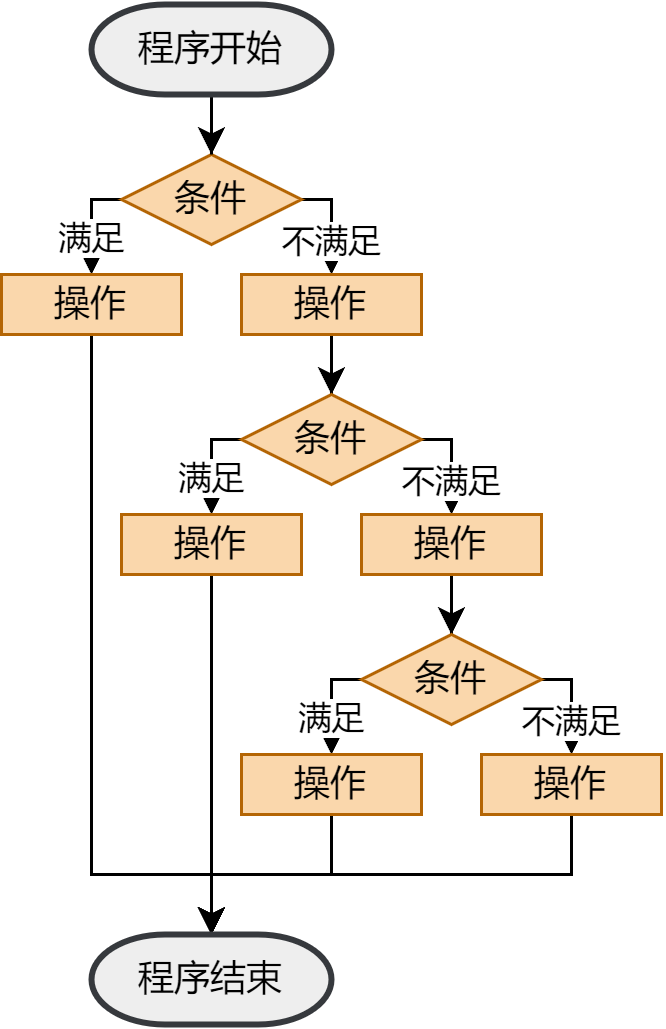
\includegraphics[width=0.4\textwidth]{../images/generalized_parts/03_if_elseif_else_300.png}
    \caption{\lstinline@if@-\lstinline@else@ 嵌套实现多路分支}
\end{figure}
\subsection*{\lstinline@switch@-\lstinline@case@ 结构}
\lstinline@switch@-\lstinline@case@ 结构是一种在特定情况下可以方便地实现多路选择的选择结构。它的基本语法是
\begin{lstlisting}
    switch (<整型数据>) {
        case <字面量>: //判断分支
            <操作>
            break; //break并非必需,但请注意后果
        case <字面量>: //判断分支
            <操作>
            break;
        default: //默认情况
            <操作>
            break; //break并非必需,尤其对于最末的case而言
    }
\end{lstlisting}\par
\lstinline@switch@\lstinline@case@ 结构与 \lstinline@if@ 结构不同,它的判断是通过``匹配''进行的。\par
\lstinline@switch@ 块中的每个 \lstinline@case@ 都是一个标签,能对某个位置进行标记。\lstinline@switch@ 跟随的整型数据将会去匹配每个\lstinline@case@ 标签后的字面量\footnote{其实不光是字面量,所有常量表达式都是可以用的。}。一旦匹配到了合适的字面量,程序就会从本句开始顺序执行。\par
现在我们要输入一个1\~{}6之间的正整数,并输出它的英文(one, two, \ldots);如果输入不是1\~{}6之间的正整数,就什么也不做。我们可以按照下面这个使用 \lstinline@switch@-\lstinline@case@ 结构的代码来实现这个功能。
\begin{lstlisting}
    int num; //定义待输入变量,注意必须用整型、字符型或布尔型
    cin >> num; //输入num的值
    switch (num) {
        case 6: //case可以从1到6,也可以从6到1,也可以打乱顺序,对应即可
            cout << "six" <<endl; //如果num匹配6,就从这里开始顺序执行
            break; //用break来退出switch块
        case 5:
            cout << "five" << endl; //如果num匹配5,就从这里开始顺序执行
            break;
        case 4:
            cout << "four" << endl;
            break;
        case 3:
            cout << "three" << endl;
            break;
        case 2:
            cout << "two" << endl;
            break;
        case 1: //最末的case可以不加break
            cout << "one" << endl;
    }
\end{lstlisting}
可以看出,这样写要比用 \lstinline@else if@ 然后加一众 \lstinline@num==@ 的方式要简洁一些。读者可以自行测试这段代码,看看效果。\par
\lstinline@switch@-\lstinline@case@ 结构有一个特性,叫做\textbf{穿透效应(Fallthrough behavior)}。因为 \lstinline@case@ 只是一个标签,不能起到退出 \lstinline@switch@ 结构的作用,所以如果在写每个 \lstinline@case@ 之后不加以 \lstinline@break@ 的话,程序将会继续运行下一个 \lstinline@case@、再下一个 \lstinline@case@,至到遇到一个退出语句或者运行到 \lstinline@switch@ 的末尾为止。\par
举个例子来说,如果上面的代码不加 \lstinline@break@ 的话,程序运行的结果将是这样的\footnote{本书默认:键盘输入的内容用黑体标识,程序输出的内容不用黑体。换行符不单独显示,行末空格和回车也忽略掉。如有特殊情况,会特别说明。}:\\\noindent\rule{\linewidth}{0.2pt}\texttt{
\textbf{4}\\
four\\
three\\
two\\
one
}\\\noindent\rule{\linewidth}{0.2pt}
而加上了 \lstinline@break@ 之后就会得到这样的运行结果:\\\noindent\rule{\linewidth}{0.2pt}\texttt{
\textbf{4}\\
four
}\\\noindent\rule{\linewidth}{0.2pt}\par
我们还可以做合并标签的操作,这个效果相当于``如果 \lstinline@<整型数据>@ 匹配了 \lstinline@<字面量1>@ \textbf{或者} \lstinline@<字面量2>@,就从这里开始执行''。\par
举个例子,某个百分制的成绩根据分数划定等级,90\~{}100分定为A,80\~{}89分定为B,70\~{}79分定为C,60\~{}69分定为D,0\~{}59分定为E。我们可以用 \lstinline@switch@-\lstinline@case@ 结构来实现输入成绩,输出等级的操作。\par
首先思考一下我们该用什么思路。如果直接按照100分制来写 \lstinline@case@ 的话,那么我们要为 \lstinline@score@ (代表分数的整型变量)变量写100个 \lstinline@case@,这个实在太麻烦了。即便考虑到可以用 \lstinline@default@ 来表示60分以下的情况,我们也要为 \lstinline@60@ 及以上的分数写41个 \lstinline@case@。这还不如用 \lstinline@if@-\lstinline@else@ 呢,好歹这种方式可以表示范围。\par
为了简化我们的代码,我们可以取个巧:用 \lstinline@score/10@ 来匹配数据(还记得吗,整型变量的除法是自动截尾的)。这样我们就只需为 \lstinline@6@, \lstinline@7@, \lstinline@8@, \lstinline@9@ 和 \lstinline@10@ 来写 \lstinline@case@ 了。\par
\begin{lstlisting}
    switch (score / 10) { //用score/10来匹配数据
        case 10:
        case 9: //合并9和10两个case,如果匹配9或10都从这里开始顺序运行
            cout << "A" << endl; //输出A
            break; //不要忘记break,否则还会顺序执行后面的代码
        case 8:
            cout << "B" << endl;
            break;
        case 6: //打乱case的顺序?完全没问题,编译器不会误解的
            cout << "D" << endl;
            break;
        case 7:
            cout << "C" << endl;
            break;
        default: //如果以上均不匹配,就应该是E等了吧
            cout << "E" << endl;
            break; //最末case可不加break,加了也行
    }
\end{lstlisting}
